%% LyX 2.3.6.1 created this file.  For more info, see http://www.lyx.org/.
%% Do not edit unless you really know what you are doing.
\documentclass[12pt,phd]{psuthesis}
\usepackage{lmodern}
\usepackage{lmodern}
\usepackage[T1]{fontenc}
\usepackage[latin9]{inputenc}
\setcounter{secnumdepth}{3}
\setcounter{tocdepth}{3}
\synctex=-1
\usepackage{amsmath}
\usepackage{amssymb}
\usepackage{graphicx}
\usepackage{setspace}
\usepackage{microtype}
\setstretch{1.24}

\makeatletter

%%%%%%%%%%%%%%%%%%%%%%%%%%%%%% LyX specific LaTeX commands.
%% Because html converters don't know tabularnewline
\providecommand{\tabularnewline}{\\}
%% A simple dot to overcome graphicx limitations
\newcommand{\lyxdot}{.}


\@ifundefined{showcaptionsetup}{}{%
 \PassOptionsToPackage{caption=false}{subfig}}
\usepackage{subfig}
\makeatother

\begin{document}
% !TEX root = ../JustinRodriguez-Dissertation.tex

\chapter{Electric field induced metallic behavior in thin crystals of ferroelectric
$\ensuremath{\alpha}\textrm{-In}_{2}\textrm{Se}_{3}$\label{chapter:FeSm-FET}}

\section{Introduction and background}

\section{Device manufacture}

Thin crystals of $\textrm{\ensuremath{\alpha}-In}_{2}\textrm{Se}_{3}$
were grown by a modified Bridgman method. Transport measurements were
carried out on both bulk and thin mechanically exfoliated crystals.
For bulk resistivity measurements, silver paint was used to form conductive
terminals. In-plane resistivity measurements were carried out using
a hall bar pattern along the longest axis of the bulk crystal. For
out-of-plane measurements, to ensure a fresh surface, the previous
leads were removed with a razor before new leads were added on. A
modified four-point pattern was used to accommodate the thin c-axis
of the crystal: a current lead was placed in the center of the crystal
on the opposing sides of the c-axis with a voltage lead encircling
each current lead.

Flakes of thin crystals of $\textrm{\ensuremath{\alpha}-In}_{2}\textrm{Se}_{3}$
on $\textrm{Si:P/Si}\textrm{O}_{2}$ were manufactured using mechanical
exfoliation as described in \ref{subsec:Mechanical-flake-exfoliation}.
Flakes were identified under an optical microscope and atomic force
microscopy was used to establish a rough color code to judge the thickness
of the flakes. Below 20nm, flakes were observed with the same shade
of blue but appeared increasingly transparent for as thickness decreased.
To promote better van der Walls adhesion of the flake to the substrate,
the latter was first cleaned in Nanostrip, Acetone, 2-Proponal, and
DI-water, before flake exfoliation, and the substrate was heated to
100C while in contact with the tape prior to the final removal. After
optical identification, flake-substrates were kept in a drybox, or
later in vacuum, to avoid water contamination and oxidation. 

\begin{figure}
\begin{centering}
\subfloat[Hall bar schematic]{\begin{centering}
\includegraphics{Figures/Hall_bar}
\par\end{centering}
}
\par\end{centering}
\begin{centering}
\subfloat[Sample A]{\includegraphics[width=1.35in]{Figures/JR200115_11}

}~~~\subfloat[Sample B]{\includegraphics[width=1.35in]{Figures/JR200115_17}}~~~\subfloat[Sample C]{\includegraphics[width=1.35in]{Figures/JR190919_03}}~~~\subfloat[Sample D]{\includegraphics[width=1.35in]{Figures/JR190815_04}}
\par\end{centering}
\caption{Device images\label{fig:In2Se3-Device-images}}

(a) Schematic of the Hall bar device with used in flake measurements.
(b-e) Optical images of sample devices following this design with
10 $\mu m$ scale bars.
\end{figure}

\begin{table}
\begin{centering}
\begin{tabular}{|c|c|c|c|c|c|}
\hline 
Sample & $t\,(nm)$ & $L_{volt}\,\left(\mu m\right)$ & $L_{current}\,\left(\mu m\right)$ & $w\,\left(\mu m\right)$ & Device pattern\tabularnewline
\hline 
\hline 
A & 20 & 2 & 12 & 5 & four-point probe\tabularnewline
\hline 
B & 13 & 4 & 16 & 30 & four-point probe\tabularnewline
\hline 
C & 110 & 5 & 15 & 10 & Hall bar\tabularnewline
\hline 
D & 110 & 2 & 12 & 9 & Hall bar\tabularnewline
\hline 
\end{tabular}
\par\end{centering}
\caption{Device parameters\label{tab:In2Se3-Device-parameters}}

Physical dimensions of the $\ensuremath{\alpha}\textrm{-In}_{2}\textrm{Se}_{3}$
crystals used in the sample devices and the lead configuration. $L_{volt}$
and $L_{current}$ are the shortest distances between the voltage
and current leads, $w$ the channel width of the crystal, and $t$
the thickness of the crystal. 
\end{table}

Flakes of crystal were made into four-point probe and Hall bar FET
devices using photolithography and e-beam metal deposition. Similar
to many other van der Waals chalcogenide materials, $\textrm{In}_{2}\textrm{Se}_{3}$
is sensitive to the alkali (base) developers used in many photodevelopment
processes.\cite{choi2011su8protective,choi2008aprotective} Initial
Hall bar devices with thinner crystal flakes were completely inoperative
after manufacture, while thicker devices showed substantial Schottky
barriers on various contacts. Milling away crystal material between
the lithography and metal evaporation produced better contacts but
was inconstant and only worked with thicker devices. To circumvent
this effect, we modified our lithography step to only allow solvent
developers in contact with the flake material, with the procedure
described in section \ref{subsec:PMMA+PMGI+SPR}. 5 nm of titanium
and 45 nm of gold was evaporated using either a Lab-18 Thin Film Deposition
System (Kurt J. Lesker Co.) or a Temescale FC2000 (Ferrotec). The
excess material was removed using the solvent Remover-PG (Microchem).
Figure \ref{fig:In2Se3-Device-images} shows the layout and optical
images of the devices measured in this chapter, table \ref{tab:In2Se3-Device-parameters}
the corresponding parameters of those devices.

\section{Optical crystal measurements}

Indium and selenium can form a variety of compounds, and the growth
process is complicated and may result in materials of mixed structures,
see section \ref{subsec:In-Se-compounds}.\cite{liu2019atomically}
Because of this is important to establish the stoichiometry and lattice
stacking of the crystals used in our devices. X-Ray diffraction displayed
peaks corresponding to the $R3m$ or $R\bar{3}m$ space groups. Raman
showed peaks near 104, 179, and 193 $cm^{-1}$corresponding to the
$A_{1}^{\,1}$, $E^{3}$, and $A_{1}^{\,4}$ peaks of $\textrm{\ensuremath{\alpha}-In}_{2}\textrm{Se}_{3}$.\cite{liu2019atomically,balakrishnan2018epitaxial}
Photoluminescence (PL) showed an energy gap of 1.4 $eV$, consistent
with previous optical measurements.\cite{balakrishnan2018epitaxial}
Finally, angle-resolved second harmonic generation (SHG) showed a
six-fold symmetry establishing the material as stacking in a $R3m$
(166) space group lattice.\cite{hou2019resistive,dai2020intrinsic,xiao2018intrinsic}
Figure \ref{fig:In2Se3-Optical-measurements} shows the Raman, PL
, and SHG measurements performed on exfoliated flakes of crystal on
$\textrm{Si:P/Si}\textrm{O}_{2}$ wafer chips.

\noindent 
\begin{figure}
\begin{centering}
\subfloat[Raman]{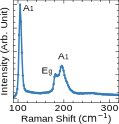
\includegraphics{Figures/In2Se3_Raman_txt}

}~~\subfloat[Photoluminescence]{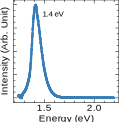
\includegraphics{Figures/In2Se3_Photoluminescence_txt}}~~\subfloat[Second Harmonic Generation]{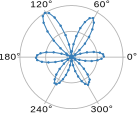
\includegraphics{Figures/In2Se3_angled_SHG_txt}

}\caption{Optical measurements of $\textrm{\ensuremath{\alpha}-In}_{2}\textrm{Se}_{3}$.\label{fig:In2Se3-Optical-measurements} }
\par\end{centering}
Raman (a), photoluminescence (b), and angle-resolved SHG (c) of exfoliated
$\textrm{\ensuremath{\alpha}-In}_{2}\textrm{Se}_{3}$ flakes.
\end{figure}


\section{FET measurements}

Flakes of thin crystal were manufactured into Hall bar and four-point
probe FET devices for electronic characterization, both on conductive
substrates of doped silicon with an insulating layer of 300nm thermally
grown $\textrm{Si:P/Si}\textrm{O}_{2}$. Source-drain current $I_{D}$
was measured against voltage bias $V_{DS}$ from 0 to 5 V, and separately
for 0 to -5 V, for fixed back gate voltages. Gate voltages were fixed
in 25 V intervals from -75 V to 75 V for each sequence. Figure \ref{fig:In2Se3-SampleA-I_DSvV_DS}
shows the data for sample A. The rapid change in $I_{D}$ around 0
V is indicative of two back-to-back Schottky diodes, see section \ref{sec:Metal-Semiconductor-Metal-conduc}.
Samples B and C showed a similar measurement with both the increasing
and decreasing $V_{DS}$ bias for fixed gate voltages, figures \ref{fig:Sample-B-IDvsVDS}
and \ref{fig:Sample-C-IDvsVDS}. None of the samples measured were
seen to saturate within $\pm10$ V for any gate bias. The lower $I_{D}$
for negative $V_{DS}$ bias than positive is typical of n-type semiconductors,
which is seen in most reports of $\textrm{\ensuremath{\alpha}-In}_{2}\textrm{Se}_{3}$\cite{island2015gatecontrolled,1986electrical}.
Sample A $V_{DS}$ bias was cycled from 0 V, 10 V, -10V, to 0 V, forming
asymmetric hysteresis in the current. The switching behavior is similar
to previous reports of $\textrm{\ensuremath{\alpha}-In}_{2}\textrm{Se}_{3}$
transistors, where the ferroelectric polarization field is thought
to modify the Schottky barrier between the material and the metal
leads.<TODO Refs>

\begin{figure}
\begin{centering}
\subfloat[$I_{D}\left(V_{DS,\uparrow},\,V_{G,\uparrow}\right)$]{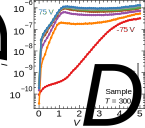
\includegraphics{Figures/JR200115_11/JR200115_11_300K_IDvVDS-positive_VG-increasing_log_txt}}~~\subfloat[$I_{D}\left(V_{DS,\downarrow},\,V_{G,\uparrow}\right)$]{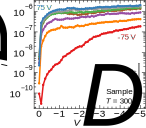
\includegraphics{Figures/JR200115_11/JR200115_11_300K_IDvVDS-negative_VG-increasing_log_txt}}~~\subfloat[$I_{D}\left(V_{DS,\updownarrow},\,V_{G,\uparrow}\right)$]{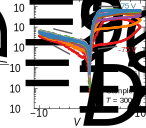
\includegraphics{Figures/JR200115_11/JR200115_11_300K_IDvVDS-loop_VG-increasing_log_txt}

}
\par\end{centering}
\begin{centering}
\subfloat[$I_{DS}\left(V_{DS,\uparrow},\,V_{G\downarrow}\right)$]{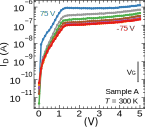
\includegraphics{Figures/JR200115_11/JR200115_11_300K_IDvVDS-positive_VG-decreasing_log_txt}}~~\subfloat[$I_{D}\left(V_{DS,\downarrow},\,V_{G,\downarrow}\right)$]{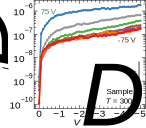
\includegraphics{Figures/JR200115_11/JR200115_11_300K_IDvVDS-negative_VG-decreasing_log_txt}}~~\subfloat[$I_{D}\left(V_{DS,\updownarrow},\,V_{G,\downarrow}\right)$]{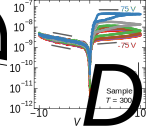
\includegraphics{Figures/JR200115_11/JR200115_11_300K_IDvVDS-loop_VG-decreasing_log_txt}

}\caption{Sample A: $I_{D}\left(V_{DS}\right)$\label{fig:In2Se3-SampleA-I_DSvV_DS}}
\par\end{centering}
$I_{D}\left(V_{DS}\right)$ of Sample A with increasing (a \& d) and
decreasing (b \& e) $V_{DS}$. (c \& f) hysteresis in the current
as $V_{DS}$ is cycled from 0 V, 10 V, -10 V, to 0 V. (a - c) are
taken while $V_{G}$ is taken in increasing fixed 25 V intervals and
(d - f) decreasing. All measurements were done at 300 K.
\end{figure}

FET transistor transfer curves $I_{D}$ measured against back-gate
bias $V_{G}$ was also measured. Each measurement was performed with
a fixed $V_{DS}=.1V$, with the $V_{G}$ cycled from 0 V, to -75 V,
75 V, -75 V, to 0 V, shown in figure \ref{fig:In2Se3-Sample-A-loops}.
For clarity, only the data between -75 V, 75 V, to -75 V is shown,
as that behavior is persistent across multiple loops. The measurement
was repeated at various, fixed temperatures from 300 K to 2-4 K, the
lowest temperature being sample dependent due to blockages in the
PPMS. For each sweep of $V_{G}$ the $I_{D}$ formed a clockwise hysteresis
loop. In all samples the width of the loop decreased with decreasing
temperature, though each sample still exhibited a finite hysteresis
at the lowest temperature. Samples B and C showed similar clockwise
hysteresis behavior, shown in \ref{fig:Sample-B-loops} and \ref{fig:Sample-C-loops}.

\begin{figure}
\begin{centering}
\subfloat[300 K]{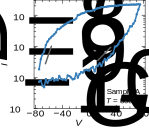
\includegraphics{Figures/JR200115_11/JR200115_11_IDvVG_300K_log_txt}}~\subfloat[200 K]{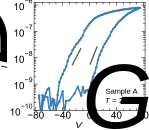
\includegraphics{Figures/JR200115_11/JR200115_11_IDvVG_200K_log_txt}}~\subfloat[150 K]{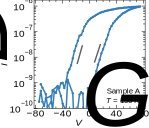
\includegraphics{Figures/JR200115_11/JR200115_11_IDvVG_150K_log_txt}

}
\par\end{centering}
\begin{centering}
\subfloat[100 K]{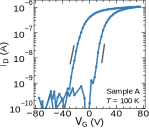
\includegraphics{Figures/JR200115_11/JR200115_11_IDvVG_100K_log_txt}}~\subfloat[50 K]{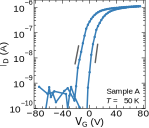
\includegraphics{Figures/JR200115_11/JR200115_11_IDvVG_050K_log_txt}}~\subfloat[2 K]{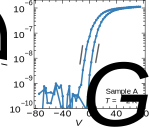
\includegraphics{Figures/JR200115_11/JR200115_11_IDvVG_002K_log_txt}

}
\par\end{centering}
\begin{centering}
\caption{Sample A: $I_{D}\left(V_{G}\right)$ transfer characteristics\label{fig:In2Se3-Sample-A-loops}}
\par\end{centering}
(a-f)$I_{D}\left(V_{G}\right)$ of Sample A at fixed temperatures
as indicated. Each was measured with $V_{DS}=0.1\,V$ as $V_{G}$
was cycled, a clockwise hysteresis loop was seen at all temperatures.
\end{figure}


\section{Discussion}

When cooled from 300 to 2 K, the bulk crystal showed an increase in
resistivity emblematic of most semiconductors, with variable range
hopping (VRH) conduction appearing below approximately 40 K. When
heating 

\begin{figure}
\begin{centering}
\subfloat[Bulk: $\rho\left(T\right)$]{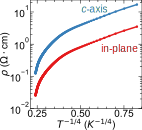
\includegraphics{Figures/In2Se3_Bulk_RT_ln}

}~~\subfloat[Sample A: $R_{DS}\left(T\right)$]{
\includegraphics{Figures/JR200115_11/JR200115_11_RDSvVG-cross-section_linear}}~~\subfloat[Sample B: $R_{DS}\left(T\right)$]{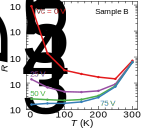
\includegraphics{Figures/JR200115_17/JR200115_17_RDSvVG-cross-section_log}}
\par\end{centering}
\begin{centering}
\subfloat[Sample C: $R_{DS}\left(T\right)$]{~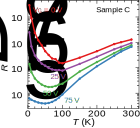
\includegraphics{Figures/JR190919_03/JR190919_03_RDSvVG-cross-section_log}~

}~~\subfloat[Sample A: magnetoconductance]{\includegraphics{Figures/JR200115_11/JR200115_11_Magnetoconductance_1\lyxdot 8K}}~~\subfloat[Sample D: Carrier density $n_{2D}\left(T\right)$]{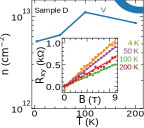
\includegraphics{Figures/JR190815_04/JR190815_04_Hall_combined}}
\par\end{centering}
\caption{Temp dependence}

Bulk
\end{figure}

\end{document}
